%%%%%%%%%%%%%%%%%%%%%%%%%%%%%%%%%%%%%%%%%
% Short Sectioned Assignment
% LaTeX Template
% Version 1.0 (5/5/12)
%
% This template has been downloaded from:
% http://www.LaTeXTemplates.com
%
% Original author:
% Frits Wenneker (http://www.howtotex.com)
%
% License:
% CC BY-NC-SA 3.0 (http://creativecommons.org/licenses/by-nc-sa/3.0/)
%
%%%%%%%%%%%%%%%%%%%%%%%%%%%%%%%%%%%%%%%%%

%----------------------------------------------------------------------------------------
%   PACKAGES AND OTHER DOCUMENT CONFIGURATIONS
%----------------------------------------------------------------------------------------

\documentclass[paper=a4, fontsize=11pt]{scrartcl} % A4 paper and 11pt font size

\usepackage[T1]{fontenc} % Use 8-bit encoding that has 256 glyphs
\usepackage{fourier} % Use the Adobe Utopia font for the document - comment this line to return to the LaTeX default
\usepackage[english]{babel} % English language/hyphenation
\usepackage{amsmath,amsfonts,amsthm} % Math packages
\usepackage[makeroom]{cancel}
\usepackage{subcaption}
\usepackage{graphicx}
\usepackage{url}

\usepackage{lipsum} % Used for inserting dummy 'Lorem ipsum' text into the template

\usepackage{sectsty} % Allows customizing section commands
\allsectionsfont{\centering \normalfont\scshape} % Make all sections centered, the default font and small caps

\usepackage{fancyhdr} % Custom headers and footers
\pagestyle{fancyplain} % Makes all pages in the document conform to the custom headers and footers
\fancyhead{} % No page header - if you want one, create it in the same way as the footers below
\fancyfoot[L]{} % Empty left footer
\fancyfoot[C]{} % Empty center footer
\fancyfoot[R]{\thepage} % Page numbering for right footer
\renewcommand{\headrulewidth}{0pt} % Remove header underlines
\renewcommand{\footrulewidth}{0pt} % Remove footer underlines
\setlength{\headheight}{13.6pt} % Customize the height of the header
\usepackage{listings}

\numberwithin{equation}{section} % Number equations within sections (i.e. 1.1, 1.2, 2.1, 2.2 instead of 1, 2, 3, 4)
\numberwithin{figure}{section} % Number figures within sections (i.e. 1.1, 1.2, 2.1, 2.2 instead of 1, 2, 3, 4)
\numberwithin{table}{section} % Number tables within sections (i.e. 1.1, 1.2, 2.1, 2.2 instead of 1, 2, 3, 4)

\setlength\parindent{0pt} % Removes all indentation from paragraphs - comment this line for an assignment with lots of text

%----------------------------------------------------------------------------------------
%   TITLE SECTION
%----------------------------------------------------------------------------------------

\newcommand{\horrule}[1]{\rule{\linewidth}{#1}} % Create horizontal rule command with 1 argument of height

\title{
\normalfont \normalsize
\textsc{Digital Pre-Distortion for ODR-DabMod} \\ [25pt] % Your university, school and/or department name(s)
\horrule{0.5pt} \\[0.4cm] % Thin top horizontal rule
\horrule{2pt} \\[0.5cm] % Thick bottom horizontal rule
}

\author{Open Digital Radio} % Your name

\date{\normalsize\today} % Today's date or a custom date

\begin{document}

\maketitle % Print the title

\section{Hardware Setup}

\begin{figure}
    \begin{subfigure}[c]{0.5\textwidth}
      \center
      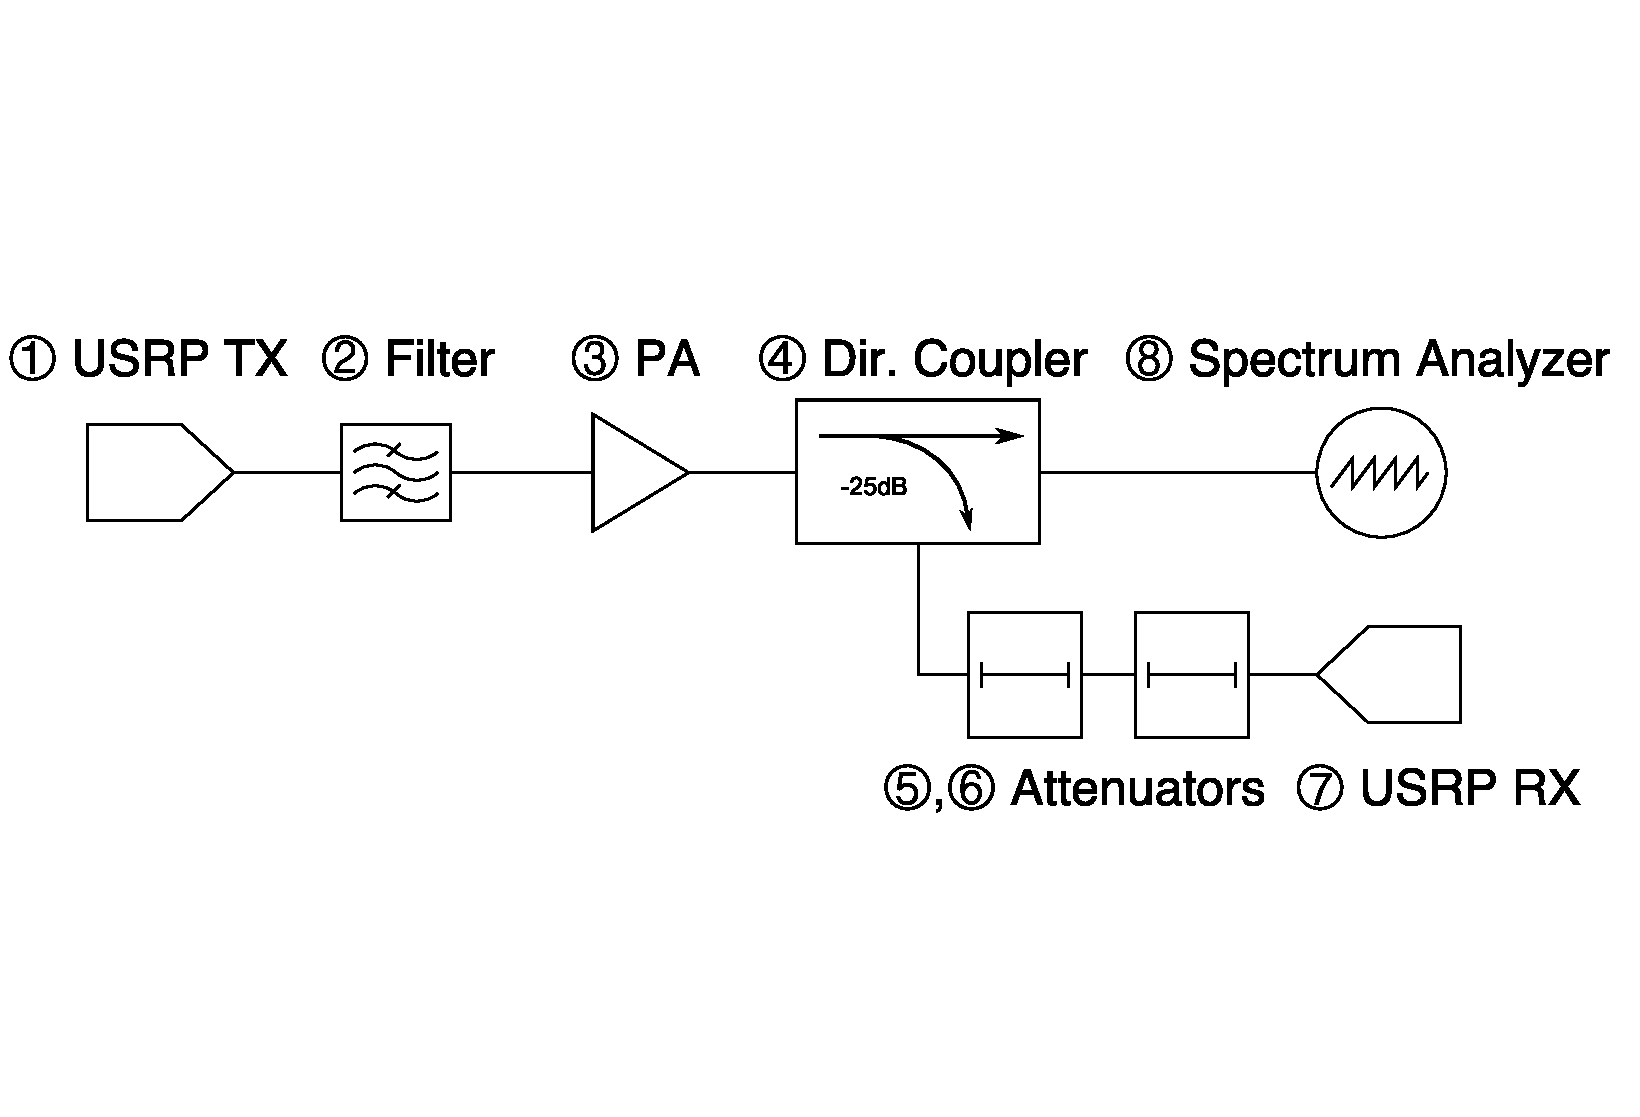
\includegraphics[width=\textwidth]{img/setup_diagram}
      \subcaption{Diagram}
      \label{fig:setup_diagram}
  \end{subfigure}%
  \begin{subfigure}[c]{0.5\textwidth}
      \center
      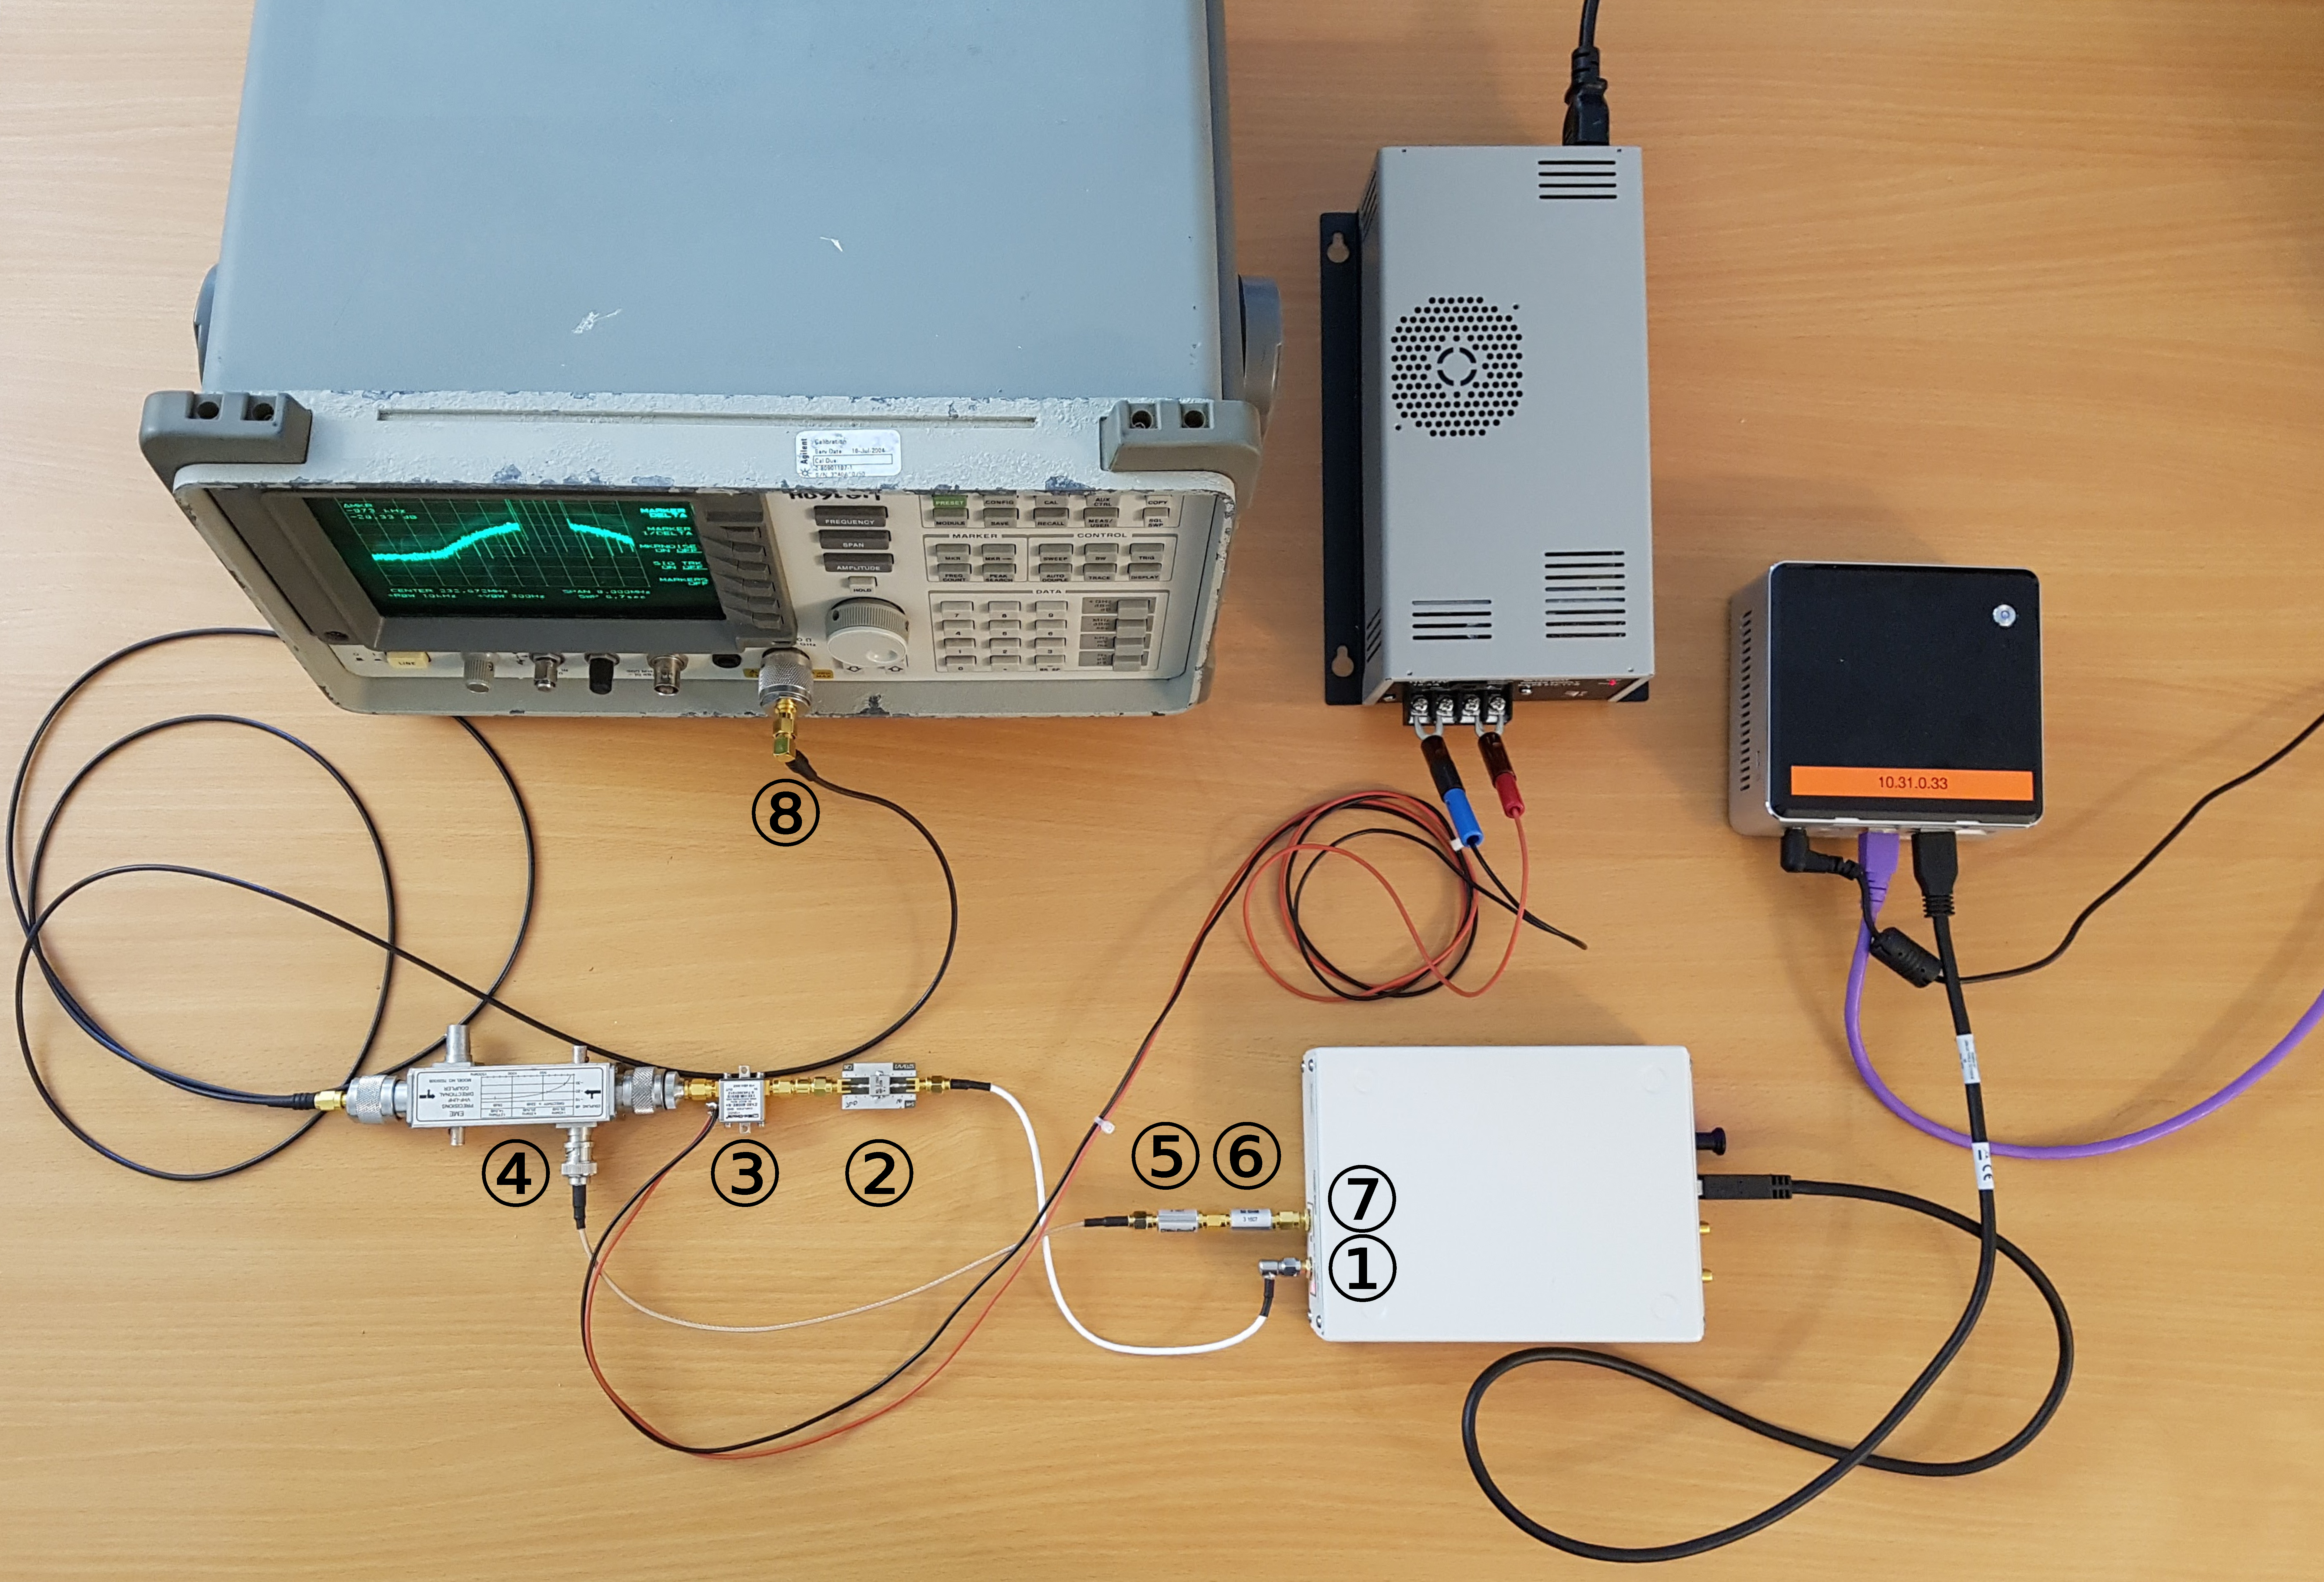
\includegraphics[width=\textwidth]{img/setup_photo}
      \subcaption{Photo}
      \label{fig:setup_photo}
  \end{subfigure}
\caption{Setup}
\label{fig:setup}
\end{figure}

Our setup is depicted in Figure~\ref{fig:setup}. We used components with the following properties:
\begin{enumerate}
    \item USRP TX (max +20dBm)
    \item Filter (190-250MHz, -3.5dB)
    \item Power amplifier (max +15dBm, +10 dB)
    \item Directional coupler (approx. -25dB @ 223MHz)
    \item Attenuator (-20 dB)
    \item Attenuator (-30 dB)
    \item USRP RX (max -15dBm)
    \item Spectrum analyzer (max +30dBm)
\end{enumerate}

It is important to make sure, that the USRP RX port does not receive too much power. Otherwise the USRP will break. Here is an example of how we calculated the maximal USRP RX input power for our case. As this is only a rough calculation to protect the port, the pre-distortion software will later automatically apply a normalization for the RX input by adapting the USRP RX gain.
$$P_{TX} + P_{PA} - P_{SP} - P_{AT} = 20dBm + 10dB -25dB -50dB = -45dBm$$

Thus we have a margin of about 30dB for the input power of the USRP RX port.


\section{Software Setup}

We assume that you already installed \emph{ODR-DabMux} and \emph{ODR-DabMod}. In order to satisfy dependencies for the pre-distortion, you can install all required python modules using conda. Alternatively you can also install the packages specified in the environment file via your preferred method. To install and use the environment via conda do following:

\begin{lstlisting}
conda env create -f dpd/environment.yml
source activate dab
\end{lstlisting}


\section{Use the pre-distortion}

Run the multiplexer and the modulator:

\begin{lstlisting}
ODR-DabMux/src/odr-dabmux ../simple.mux
ODR-DabMod/odr-dabmod dpd/dpd.ini
\end{lstlisting}

The script uses automatic gain control for both TX and RX gain, to get both a high quantization quality for the most frequent amplitude regions and a high enough back-off so the peaks are also quantized correctly. This means that the output power will stay at the same level, but the script may change TX gain to trade it with digital gain and also change RX gain. \\

As a first test you can run the main script without parameters. It preserves the output power and generates all available visualization plots in the newly created logging directory \path{/tmp/dpd_<time_stamp>}. To run it do following:

\begin{lstlisting}
cd dpd
python main.py
\end{lstlisting}

Each plot is stored to the logging directory under a filename containing its time stamp and its label. Following plots are generated chronologically:
\begin{itemize}
    \item ExtractStatistic: Extracted information from one or multiple measurements.
    \item Model\_AM: Fitted function for the amplitudes of the power amplifier against the TX amplitude.
    \item Model\_PM: Fitted function for the phase difference of the power amplifier against the TX amplitude.
    \item adapt.pkl: Contains the settings for the pre-distortion. To load them again without further measurements, you can use \path{apply_adapt_dumps.py}.
    \item MER: Constellation diagram used to calculate the modulation error rate.
\end{itemize}

After the run you should be able to observe that the peak-shoulder difference decrease on your spectrum analyzer, similar to Figure~\ref{fig:shoulder_measurement}. \\

\begin{figure}
    \begin{subfigure}[c]{0.5\textwidth}
      \center
      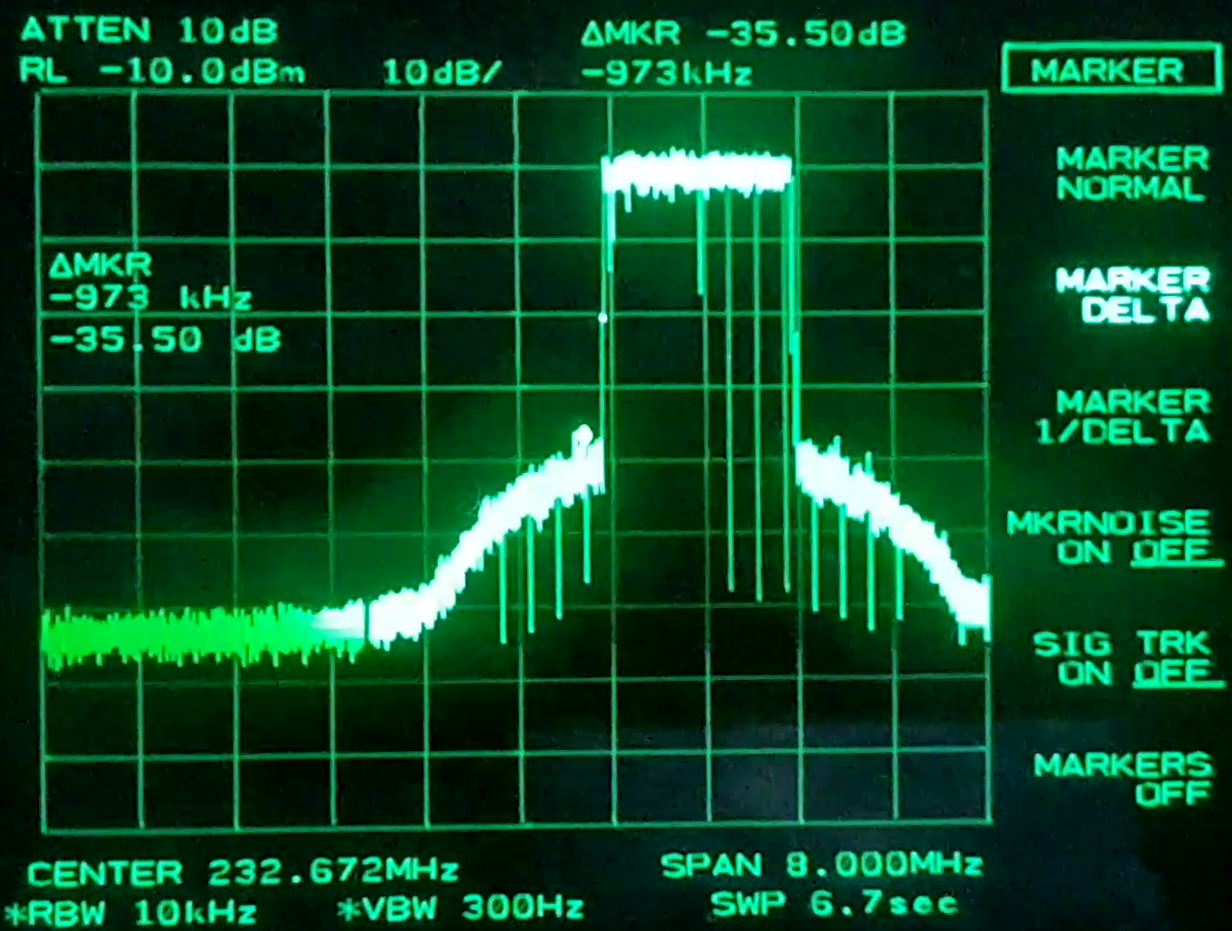
\includegraphics[width=0.9\textwidth]{img/shoulder_measurement_before}
      \subcaption{Before}
  \end{subfigure}%
  \begin{subfigure}[c]{0.5\textwidth}
      \center
      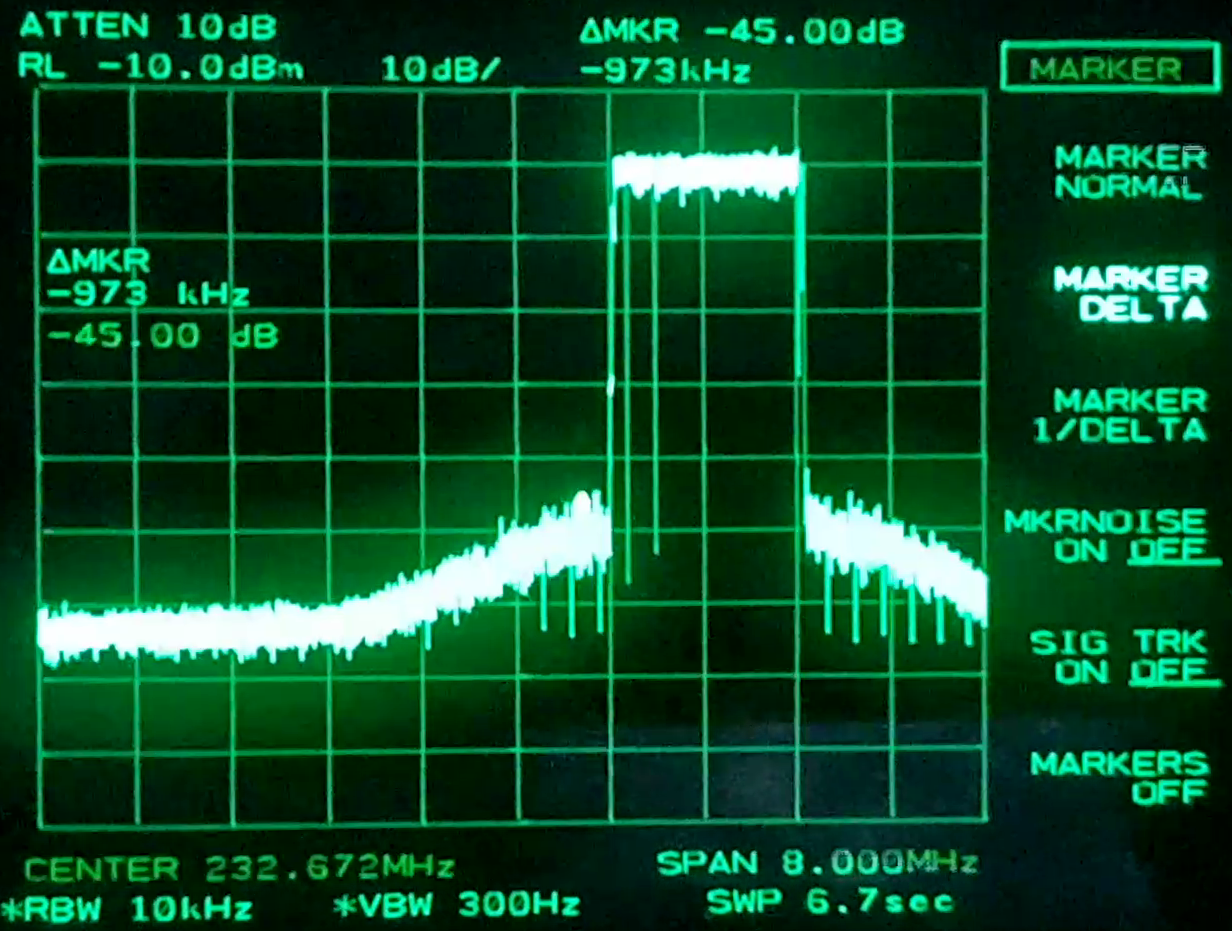
\includegraphics[width=0.9\textwidth]{img/shoulder_measurement_after}
      \subcaption{After}
  \end{subfigure}
\caption{Shoulder Measurement}
\label{fig:shoulder_measurement}
\end{figure}

Now see what happens if you apply the pre-distortions for different TX gains. You can either set the TX gain before you start the pre-distortion or using the command line option \texttt{-{}-txgain gain}. You can also try to adjust other parameters. To see their documentation run \texttt{python main.py -{}-help}

\end{document}
